\documentclass[11pt,a4paper]{article}

\usepackage[applemac]{inputenc}
\usepackage{latexsym}
\usepackage{graphicx}
\usepackage[francais]{babel}
\usepackage{amsmath,amssymb}
\usepackage{pstricks,pst-plot}
\usepackage{calc}
\usepackage{multicol}
\usepackage{fancyhdr}
\usepackage{lastpage}
\usepackage[T1]{fontenc}
\usepackage[top=3.5cm, bottom=2.5cm, left=1.5cm, right=1.5cm]{geometry}
\usepackage{stmaryrd}
\usepackage{float}
\pagestyle{plain}
\usepackage{epstopdf}
\usepackage{stmaryrd} 


\title{Programming Assignment 1 \\ From planning to reinforcement learning}
\author{Mathurin \textsc{Massias} \and Cl�ment \textsc{Nicolle}}
\date{\today} 

\begin{document}
\maketitle

\section{Simulated trajectories and estimation of value function}
\hspace{-6mm}The MDP here is :
\begin{itemize}
	\item State space: $X = \left[ 0; M\right] \cap \mathbb{N}$
	\item Action space: $A(x) = \left[ 0; M-x\right] \cap \mathbb{N}$
	\\
\end{itemize}
We are in the case of an infinite-horizon discounted MDP. The criterion we will try to maximize is the discounted sum of the weekly reward.
\\The transition and reward formulas given are explained below :
\\ At a given week, the shop owner has what he had last week, plus what he received (and this sum cannot be greater than the maximum he can stock), minus what he sold, and he cannot sell more than he has, so this difference cannot be negative.
\\The reward at a given week is equal to: minus the fix cost of delivery (if he orders), minus the cost of his command, minus maintenance cost, plus the sales.

\section{Policy evaluation}
\hspace{-6mm}We wrote three functions:
\\- pol\_eval\_1(pi, P, R, gamma) computes V using the matricial equation $V^{\pi} = R + \gamma PV^{\pi}$, which leads to $V^{\pi} = (I - \gamma P)^{-1} R$. In these equations $R$ and $P$ are not the general 2D and 3D matrices, but the 1D and 2D matrices associated to a given policy $\pi$ : $R = R(x, \pi(x))$ and $P = P(x, y, \pi(x))$.
\\- pol\_eval\_2(MCn,n,V0,pi,D,M,K,h,c,pr,gamma) computes an estimation of $V$ using a Monte-Carlo method (with MCn simulations) for each coordinate. It is time-consuming, converges slowly (in $\sqrt{MCn}$ by Central limit theorem), and does not provide an exact value of $V^{\pi}$.
\\- pol\_eval\_3(pi, P, R ,gamma, n\_it) computes $V^{\pi}$ using n\_it iterations of the Bellman operator. Same here, $P$ and $R$ are adapted to the peculiar policy $\pi$.


\section{Value iteration, policy iteration}
\hspace{-6mm}\textit{For real code see VI.m and PI.m files}.
%\\Pseudo code for policy iteration :
%\begin{verbatim}
%start at any pi = pi_0
%for i = 1, ..., N_it
%    evaluate V_pi
%    compute Q(x,a) = R(x,a) + gamma * sum_y P(x,y,a) V_pi (y)
%    set pi(x) =arg max Q(x,a) (over a) (improvment)
%end for
%return pi
%\end{verbatim}
%%
%Pseudo code for value iteration:
%\begin{verbatim}
%start at any V = V_0
%for i = 1, ..., N_it
%    compute Q(x,a) = R(x,a) + gamma * sum_y P(x,y,a) V(y)
%    set V = max Q(x,a) (over a) (improvment)
%end for
%return pi(x) = arg max Q(x,a) (over a)
%\end{verbatim}
%
%
\\[5mm]\textbf{Question 1:} Both VI and PI give $\pi^* = (10, 9, 8, 7, 0, ...., 0)^T$. So there is sort of a "threshold" : whenever stocks goes under 4 units, the owner must refill to get 10 units. Otherwise he does nothing. It is a balance between the risk of being short on product and missing sales, and the cost of maintenance + the cost of order.
\\[3mm]\textbf{Question 2 : }Using the arbitrary number of 500 iterations, PI using matricial evaluation takes approx 0.3 s, and so does VI. PI using Bellman operator takes 1.5 s. However, we saw that PI needed less iterations to converge, both for $V$ and $\pi$. 
\\[5mm]In terms of iterations, PI (using matricial evaluation) converges must faster than VI (i.e. in 5 iterations), both for $\pi$ and $V$.
%
\begin{figure}[H]
\centering
\noindent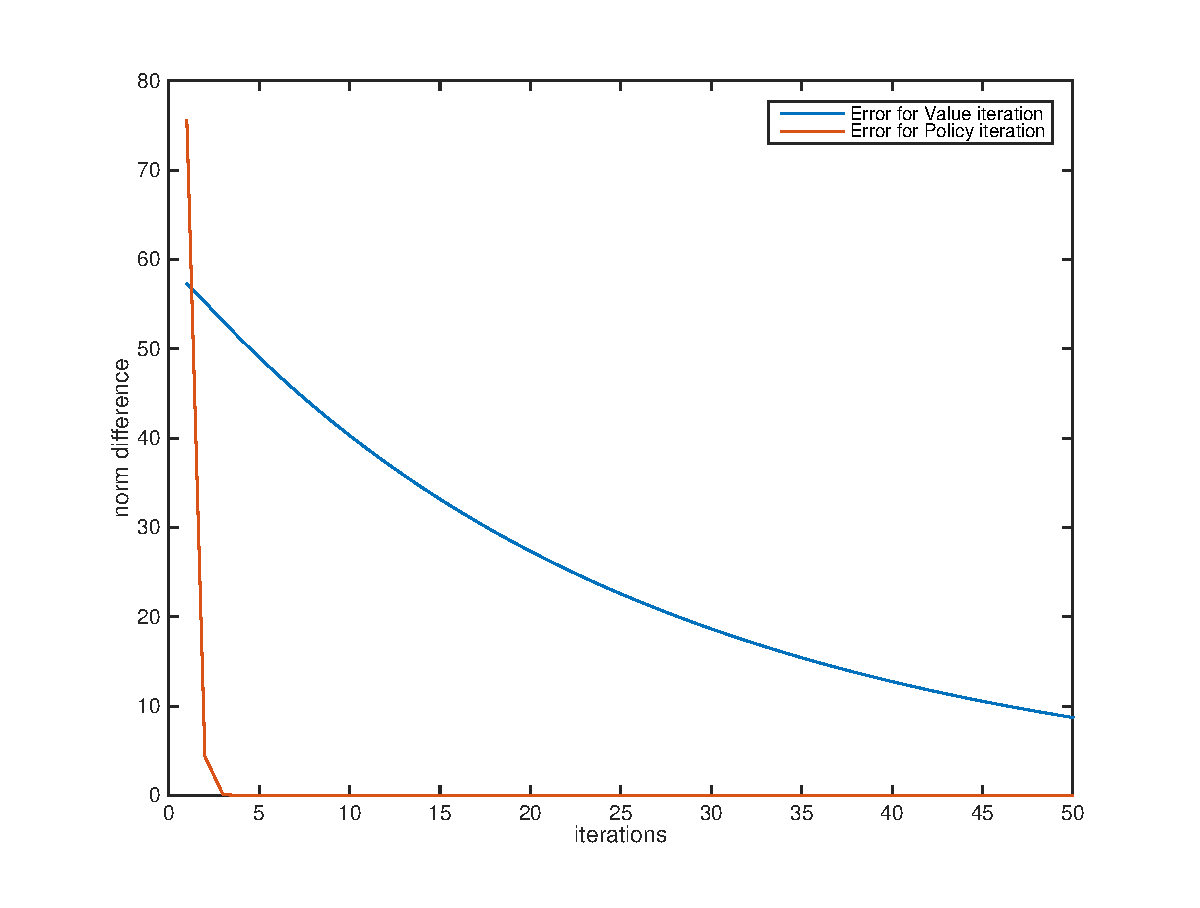
\includegraphics[scale=0.6]{Convergence_VIPI.eps}
\caption{Convergence of $V$ after $k$ iterations of PI and VI algorithms}
\end{figure}

%
\begin{figure}[H]
\centering
\noindent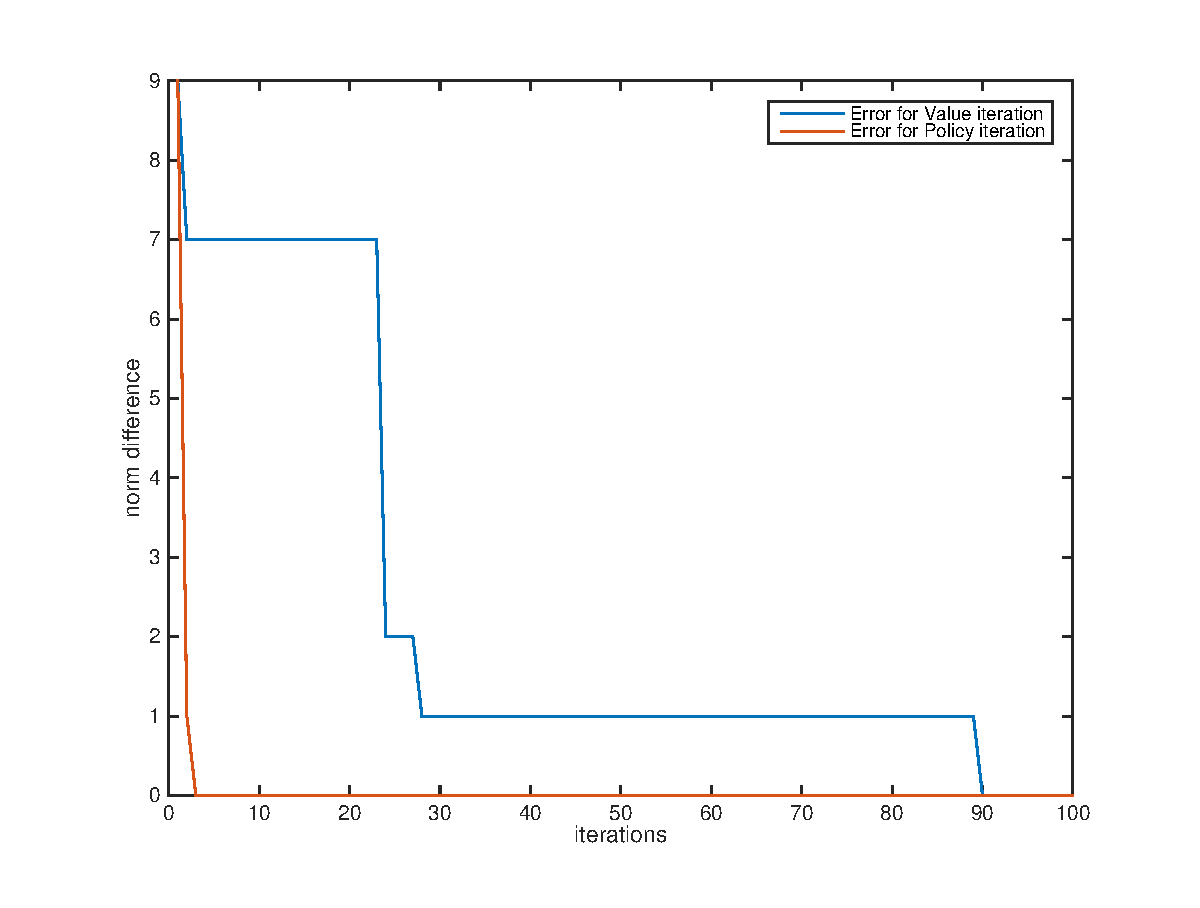
\includegraphics[scale=0.6]{Convergence_VIPI_2.eps}
\caption{Convergence of $\pi$ after $k$ iterations of PI and VI algorithms}
\end{figure}%
%

\section{Q-Learning}
\hspace*{-6mm}\textbf{Question 3} : \textit{See Qlearning.m}
\\We saw in class that the sum of the learning rate needs to be divergent, while the sum of its square needs to be convergent. In order not to erase at each iteration what we have already learned, we took $\eta_i = 1/(i+10)$.
\\Q-learning computations take around 100 s for 30,000 episodes and 200 terations.
\\In this problem, there is no terminal state. So for each episode, we made a learning through 200 weeks (we have $\gamma^{200} = 0.018$, which is rather small).
\\Here, although we do not know $D$, we observe its realisations for the demand. So, to check our results, we can compute the optimal policy for this demand using VI or PI. We then know the policy we have to find should be : $\pi^* = (10, 9, 8, 7, 0, ...., 0)^T$ here.
\\After 30 000 episodes, Q still doesn't reach its final form. But we find $\pi = (10, 9, 10, 7, 0, 0, 0, 6, 0, 1, 2, 1, 0, 0, 0, 0)^T$, which is not the final optimal policy, but it gets closer to it by increasing the number of episodes.
\\The problem is that a small variation of convergence for Q can have a great impact on the policy, because the optimal policy is related to arg max of a line of $Q$, which can change significantly if $Q$ changes just a little bit.


\end{document}